\section{Classification}

Goal: $\pi_j(x) = \mathbb{P} \eckigeklammer{Y=j | X=x}$ for all classes $1,\dots,J$.

\vspace{5pt}

\fat{Bayese Classifier}
$\mathcal{C}_B (x) = \argmax_{0 \leq j \leq J-1} \pi_j (x)$. More generally: $\mathcal{C}_B (x) = \argmin_{0 \leq k \leq J-1} \sum_{j=0}^{J-1} \mathcal{L}(j,k) \pi_j (x)$ ($\mathcal{L}(j,k)$ is the loss/cost of predicting $k$ but true class being $j$)

\vspace{-5pt}

\subsection{Linear Discriminant Analysis (LDA)}
Model: $(X|Y=j) \sim \mathcal{N}_p (\mu_j,\SigmaCov)$, $\mathbb{P}[Y=j] = p_j$, $\sum_{j=0}^{J-1} p_j = 1$
Hence: $\mathbb{P}[Y=j | X=x] = \pi_j (x) = \frac{f_{X|Y=j} (x) \cdot p_j}{\sum_{k=0}^{J-1} f_{X|Y=k} (x) \cdot p_k}$
Estimating the parameters:
$\hat{\mu}_j = \frac{\sum_{i=1}^n x_i \id_{[Y_i = j]}}{\sum_{i=1}^n \id_{[Y_i = j]}} = \frac{1}{n_j} \sum_{i=1}^n X_i \id_{[Y_i = j]}$ ,
$\hat{p}_j = \frac{n_j}{n} = \frac{1}{n} \sum_{i=1}^n \id_{[Y_i = j]}$

$\hat{\SigmaCov} = \frac{1}{n-J} \sum_{j=0}^{J-1} \sum_{i=1}^n (x_i - \hat{\mu}_j) (x_i - \hat{\mu}_j)^T \id_{[Y_i = j]}$

$\hat{\SigmaCov}_j = \frac{1}{n_j -1} \sum_{i=1}^n (x_i - \hat{\mu}_j) (x_i - \hat{\mu}_j)^T \id_{[Y_i = j]}$

$\Rightarrow \hat{\mathcal{C}}_{LDA} (x) = \argmax_{0 \leq j \leq J-1} \hat{\delta}_j (x)$ where

$\hat{\delta}_j (x) = x^T \hat{\SigmaCov}^{-1} \hat{\mu}_j - \hat{\mu}_j^T \hat{\SigmaCov}^{-1} \hat{\mu}_j /2 + \log(\hat{p}_j)
= (x-\hat{\mu}_j / 2)^T \hat{\SigmaCov}^{-1} \hat{\mu}_j + \log(\hat{p}_j)$

The decision boundary is linear.
Nbr of parameters: For $a$ predictors and $b$ groups we have $a \cdot b$ mean params, $a(a+1)/2$ CovMat params, $b-1$ priors hence $a b + a(a+1)/2 + b-1$ params in total

\vspace{-5pt}

\subsection{Quadratic Discriminant Analysis (QDA)}
Model: $(X|Y=j) \sim \mathcal{N}_p (\mu_j,\SigmaCov_j)$, $\mathbb{P}[Y=j] = p_j$, $\sum_{j=0}^{J-1} p_j = 1$

$\Rightarrow \ \hat{\delta}_j (x) = - \log \klammer{\det \klammer{\SigmaCov_j}} / 2 - (x-\hat{\mu}_j)^T \SigmaCov_j^{-1} (x-\hat{\mu}_j) / 2 + \log(\hat{p}_j)$

Nbr of params: $a b$ mean params, $b a (a+1) /2$ CovMat params, $b-1$ priors, hence $ab + ab(a+1)/2 + b -1$ params in total

\vspace{-5pt}

\subsection{Logistic Regression}

\subsubsection{Binary Classification}
$\pi(x) = \mathbb{P}[Y=1|X=x]$ and $\mathbb{P}[Y=0|X=x] = 1-\pi(x)$. Model: $\log\klammer{\frac{\pi(x)}{1-\pi(x)}} = g(x)$

\vspace{5pt}

\fat{Linear Logistic Regression} $g(x) = \sum_{j=1}^p \beta_j x_j$. Use MLE to estimate params. Assume $Y_1,\dots,Y_n \stackrel{iid}{\sim} \text{Bernoulli}(\pi(x))$:
$\mathcal{L} = \prod_{i=1}^n \pi(x_i)^{Y_i} (1-\pi(x_i))^{1-Y_i}$
$\Rightarrow - \log(\mathcal{L}) = - \sum_{i=1}^n \eckigeklammer{Y_i \sum_{j=1}^p \beta_j x_{ij} - \log \klammer{1+\exp \klammer{\sum_{j=1}^p \beta_j x_{ij}}}}$


\subsubsection{Multiclass Case}
Encode multiclass problem into $J$ binary class problems: $Y_i^{(j)} = \id_{[Y_i = j]}$. Now run log reg on each class:
$\hat{\pi}_j (x) = \frac{\exp \klammer{\sum_{r=1}^p \hat{\beta}_r^{(j)} x_r}}{1 + \exp \klammer{\sum_{r=1}^p \hat{\beta}_r^{(j)} x_r}}$

$\tilde{\pi}_j(x) = \frac{\hat{\pi}_j (x)}{\sum_{k=0}^{J-1} \hat{\pi}_k (x)}$
$\Rightarrow \ \hat{\mathcal{C}} (x) = \argmax_{0 \leq j \leq J-1} \hat{\pi}_j (x)$

\vspace{-5pt}

\subsection{ROC Curve}
Binary Cl.: $\hat{Y} (x) = 1$ iff $\hat{\pi}(x) = \hat{\mathbb{P}} [Y=1 | X=x] > \theta$ for a given $\theta \in [0,1]$.
Def: Sensitivity($\theta$) = TPR = $\mathrm{\frac{TP}{P}}$, Specificity($\theta$) = $\mathrm{\frac{TN}{N}}$, 1-sp($\theta$) = FPR = $\mathrm{\frac{FP}{N}}$.
ROC Curve: Plot Sensitivity vs. 1-Specificity (TPR vs. FPR)

\vspace{2pt}

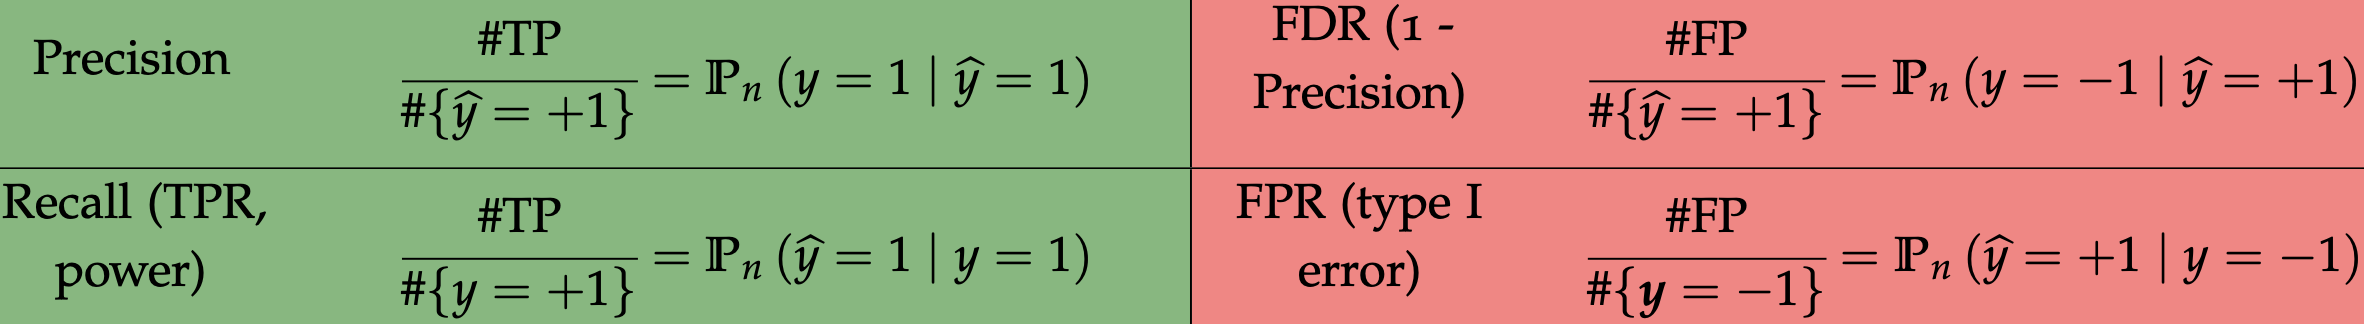
\includegraphics[width=0.495\textwidth]{Bilder/ClassificationTable.png}

% \vspace{3pt}

% Def: Sensitivity($\theta$) = TPR = $\mathrm{\frac{TP}{P}}$, Specificity($\theta$) = $\mathrm{\frac{TN}{N}}$, 1-sp($\theta$) = FPR = $\mathrm{\frac{FP}{N}}$.
% ROC Curve: Plot Sensitivity vs. 1-Specificity (TPR vs. FPR)